\documentclass[12pt,a4paper]{article}
\usepackage[margin=0.9in]{geometry}
\usepackage{graphicx}
\usepackage{booktabs}
\usepackage{array}
\usepackage{longtable}
\usepackage{hyperref}
\usepackage{fancyhdr}
\usepackage{titlesec}
\usepackage{enumitem}
\usepackage{float}
\usepackage{caption}
\usepackage{tikz}
\usetikzlibrary{shapes.geometric, arrows.meta, positioning}

\graphicspath{{images/}}

\pagestyle{fancy}
\fancyhf{}
\fancyhead[L]{P80F25 STRATBOT --- SDS}
\fancyhead[R]{DHA Suffa University}
\fancyfoot[C]{\thepage}
\renewcommand{\headrulewidth}{0.4pt}

\begin{document}

\begin{titlepage}
\centering
\vspace*{0.3cm}

{\Large \textbf{DHA Suffa University}}\\[0.2cm]
{\large Department of Computer Science}\\[0.15cm]
{\large Final Year Project}\\[1.2cm]

{\Huge \textbf{P80F25 STRATBOT}}\\[0.4cm]
{\Large \textbf{Software Design Specifications}}\\[0.8cm]

\includegraphics[width=0.42\textwidth]{dha_suffa_logo.png}\\[0.6cm]

{\large \textbf{Submitted by}}\\[0.2cm]
\begin{tabular}{l}
\textbf{Zaafir Ejaz Ur Rehman Siddiqui} (CS221222) \\
\textbf{Ebad Ahmed} (CS221217) \\
\textbf{Fatima Ather Rajput} (CS221270) \\
\end{tabular}\\[0.6cm]

{\large \textbf{Supervisor}}\\[0.15cm]
Dr. Huma Jamshed\\[0.8cm]

{\large \textbf{Document Information}}\\[0.2cm]
\begin{tabular}{ll}
Project Title & STRATBOT: AI-Based Formula 1 Race Strategy Simulation \\
Project Code & P80F25 \\
Document Name & Software Design Specifications \\
Document Version & 2.0 (Updated Implementation) \\
Document Identifier & P80F25-SDS \\
Document Status & Final \\
Author(s) & Zaafir Ejaz (Telemetry/ML), Ebad Ahmed (Data/ML), Fatima Ather Rajput (Analysis) \\
Approver(s) & Dr. Huma Jamshed \\
Issue Date & June 2026 \\
\end{tabular}

\vfill
\end{titlepage}

\tableofcontents
\newpage

\section{Introduction}
This updated SDS (v2.0) documents the \textbf{as-built} design of the delivered StratBot system (June 2026), including all FYP-I core plus implemented FYP-II elements: the 3D interactive CarCustomizer, ML deltas and customStats driving the simulation, fast-complete with visible overlay, and rich PostRace analysis.

\section{Overall System Description}
\subsection{Project Background \& Scope}
StratBot is a browser-based advisory platform for F1 strategy exploration. It combines a real-data ML pipeline (FastF1 2018-2025 + weather), a client-side high-fidelity simulation engine, live model inference, and an interactive 3D setup tool.

\subsection{System Context / Architecture}
The high-level layers (as implemented):

\begin{center}
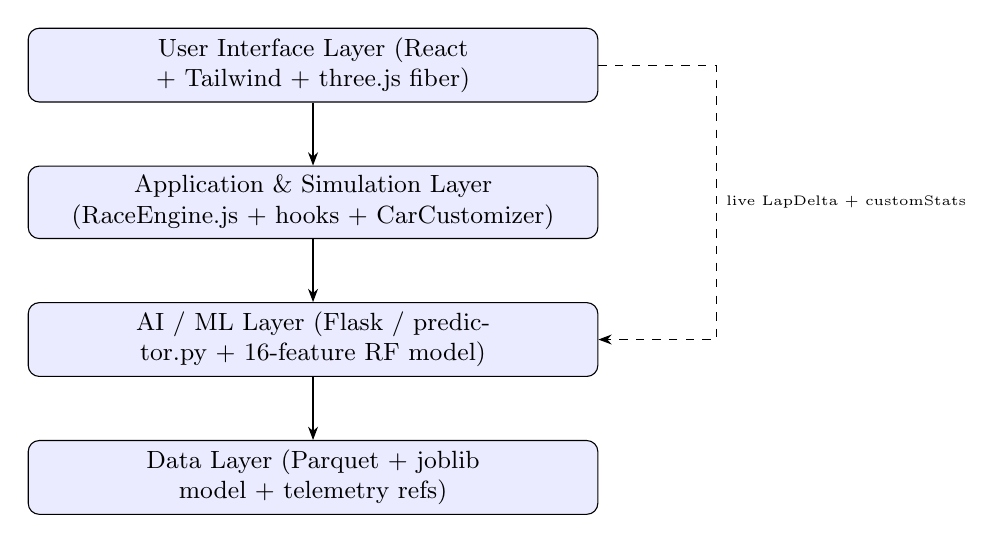
\begin{tikzpicture}[node distance=0.8cm, auto,
  block/.style={rectangle, draw, fill=blue!8, text width=7cm, text centered, rounded corners, minimum height=0.9cm, font=\small},
  line/.style={draw, -Stealth}]
  \node [block] (ui) {User Interface Layer (React + Tailwind + three.js fiber)};
  \node [block, below=of ui] (app) {Application \& Simulation Layer (RaceEngine.js + hooks + CarCustomizer)};
  \node [block, below=of app] (ai) {AI / ML Layer (Flask / predictor.py + 16-feature RF model)};
  \node [block, below=of ai] (data) {Data Layer (Parquet + joblib model + telemetry refs)};
  \draw [line] (ui) -- (app);
  \draw [line] (app) -- (ai);
  \draw [line] (ai) -- (data);
  \draw [line, dashed] (ui.east) -- ++(1.5,0) |- node[near start, right, font=\tiny] {live LapDelta + customStats} (ai.east);
\end{tikzpicture}
\end{center}

Key runtime components:
\begin{itemize}
\item \texttt{PreRaceSetup.jsx} + \texttt{CarCustomizer.jsx} (3D meshes + OrbitControls + live stats $\to$ visual + onStatsChange)
\item \texttt{RaceEngine.js} (useRaceEngine hook, refs for isFastCompleting, customCarStatsRef, burst loop with setTimeout + while(lapProgress), conditional state updates every 2 laps during fast)
\item \texttt{useStratBotModel.js} + Flask \texttt{/api/predict/lap-delta}
\item \texttt{App.jsx} (phase machine BOOT $\to$ SETUP $\to$ RACING $\to$ POST\_RACE, overlay for isFastCompleting)
\item \texttt{PostRaceSummary.jsx} (custom car stats box + ML table)
\end{itemize}

\section{External Interface Requirements}
(Identical to SRS; browser + localhost:5000/5173 + parquet on J: drive.)

\section{Functional Design}
\subsection{Use Cases (Updated)}
Primary actors: Analyst (Student/Fan), Admin (demo).

Key implemented flows:
\begin{enumerate}
\item Configure race + 3D custom car for tracked driver $\to$ Launch $\to$ (optional) interact with turns $\to$ Complete Full (visible overlay) $\to$ inspect PostRace (custom impact + ML).
\item Switch model variant / weather / compound at setup $\to$ observe different live predictions and post-race tables.
\item Fast sim auto-records ``AUTO'' decisions for any turns passed during burst.
\end{enumerate}

(Old use-case diagram from original SDS is retained in images/ for reference; actual UI flows are captured in the screenshots below.)

\section{Non-Functional Design}
Performance target for fast complete met by 120-tick / 10ms burst + ref-only heavy work + every-2-lap state refresh.

\section{Detailed System Design}

\subsection{Data Design}
\begin{itemize}
\item Primary: \texttt{f1\_model\_ready\_2018\_2025.parquet} (16 cols including weather avgs/maxes)
\item Model: \texttt{lap\_delta\_model.joblib} + \texttt{model\_meta.json} (produced by train\_export.py)
\item Runtime: in-memory telemetry refs per driver, customCarStats attached only to tracked driver object.
\end{itemize}

No traditional RDBMS (scope); Parquet + joblib as specified for FYP-I.

\subsection{UI / GUI Design (Implemented)}
All screenshots below are live captures from the running June 2026 build (not mockups).

\begin{figure}[H]
\centering
\includegraphics[width=0.98\textwidth]{ui_prerace_setup_3d.png}
\caption{Pre-Race Setup (Section 5 in original SDS) --- driver cards + fully functional embedded 3D F1 CarCustomizer. Clicking parts cycles compounds; sliders update live 3D (wing angle, tyre scale/color, engine glow) and the stats object passed to startRace().}
\end{figure}

\begin{figure}[H]
\centering
\includegraphics[width=0.98\textwidth]{ui_racing_main.png}
\caption{Racing screen with TurnNavigation (top progress bar, always-on prev/next, Complete Full, FF), LiveTimingLeaderboard, TrackMap, TelemetryCharts, ModelInsightsPanel (live prediction).}
\end{figure}

\begin{figure}[H]
\centering
\includegraphics[width=0.98\textwidth]{ui_fast_overlay.png}
\caption{Fast-complete loading overlay (z-[60] fixed inset). Text, live lap, animated progress bar. The 16ms yield + periodic setDrivers during burst ensures it is always visible and updates.}
\end{figure}

\begin{figure}[H]
\centering
\includegraphics[width=0.98\textwidth]{ui_postrace_results.png}
\caption{Post-Race (new in FYP-II) --- contains the custom ``Your Team Strategy for VER's Car'' box populated from the exact carStats chosen in the 3D customizer, plus ML comparison table and impact narrative.}
\end{figure}

\subsection{3D Car Customizer Detailed Design (FYP-II Addition)}
\begin{itemize}
\item Uses @react-three/fiber + drei (OrbitControls, Html).
\item Procedural meshes: body (box + cylinders for sidepods), front/rear wings (angled planes), nose, tyres (cylinders whose scale/color change with wear/compound), engine cone with emissive glow for power.
\item onPartClick cycles compound or opens simple numeric controls.
\item applyTeamRecommendation() computes realistic defaults per weather/track (e.g. higher aero in wet, power for overtaking tracks).
\item Live sync: stats $\to$ mesh material/scale/rotation + parent onStatsChange $\to$ PreRaceSetup state $\to$ config.carStats $\to$ RaceEngine buildInitialDrivers + predictor \_build\_row (adds biases to TyreLife, aero, power columns).
\end{itemize}

\subsection{RaceEngine Fast-Complete Design (Critical Fix)}
\begin{itemize}
\item \texttt{isFastCompletingRef} + state.
\item On click: set state + ref, setTimeout(16, runFastBurst) so React paints the overlay \textit{before} heavy work.
\item Inside burst: for(120) tick(); if not finished setTimeout(...,10).
\item Inside tick: while (lapProgress >=100) advance lap + apply custom multipliers (only for tracked driver) + weather.
\item setDrivers only every 2 laps or on finish during fast (keeps 60 fps feel for overlay text/bar).
\item Decision points during fast: auto-pick highest-prob branch and continue (no pause).
\item On leader lap > total: set raceFinished + clear isFast + transition in App to PostRace.
\end{itemize}

This design directly solves the ``black screen / no simulating fast indicator'' reported issue.

\section{References \& Appendices}
\begin{itemize}
\item Original signed SRS/SDS (P80F25) for template structure and initial diagrams (retained in images/).
\item Current stratbot/README.md, docs/PROJECT\_CONTEXT.md, TESTING.md, model\_meta.json.
\item All evaluation graphs live under stratbot/docs/evaluation/graphs/ (latest\_* versions included here).
\item 3D implementation uses three@0.167, @react-three/fiber@8, @react-three/drei@9 (legacy peer resolution via --legacy-peer-deps at install time).
\end{itemize}

\newpage
\section{Appendices -- Additional Captures \& Diagrams}

\begin{figure}[H]
\centering
\includegraphics[width=0.98\textwidth]{ui_postrace_results.png}
\caption{Full post-race view highlighting the custom car strategy box (directly driven by 3D choices) and the ML predictions captured during the run.}
\end{figure}

\begin{figure}[H]
\centering
\includegraphics[width=0.7\textwidth]{old_architecture.png}
\caption{Reference architecture diagram from original SDS (layers still match the delivered system).}
\end{figure}

\begin{figure}[H]
\centering
\includegraphics[width=0.7\textwidth]{old_usecases.png}
\caption{Reference high-level user actions from original SDS (most fully realized in current UI).}
\end{figure}

\begin{figure}[H]
\centering

\includegraphics[width=0.9\textwidth]{latest_rf_dashboard.png}
\caption{Production model performance dashboard (included for traceability of the numbers quoted throughout the documents).}
\end{figure}

\end{document}